Based on our findings in \secref{sec:07_Characterization_Extrapolation:Plane-wave_Dependence}, we use beamforming with $Q = N_\text{in}$ for the plane-wave translation method in all simulations discussed below.

% Level

Level error contour plots are shown in the top panels of \figref{fig:07_Characterization_Extrapolation:Level_Spectral_Errors}.
For the plane-wave translation method (see \figref{fig:07_Characterization_Extrapolation:Level_Errors:PWT}), we see that exterior sources experience negligible level error;
interior sources, however, are reproduced approximately $6$~dB too quietly for most microphone distances.
For the ambisonics translation method (see \figref{fig:07_Characterization_Extrapolation:Level_Errors:SRE}), we see a general trend of increasing level error with microphone distance at all source distances, although exterior sources consistently experience less severe level errors than interior ones for the same $u$, and at very large $u$ and $\gamma$ (top right corner of \figref{fig:07_Characterization_Extrapolation:Level_Errors:SRE}), the errors become less severe.
The degradation in performance with increasing microphone distance is due to the high-frequency roll-off induced by the ambisonics translation filters, as discussed in \secref{sec:07_Characterization_Extrapolation:Azimuth_Dependence}, which yields a decrease in overall level.
Taken together, these results imply that a violation of the region of validity restriction (i.e., for interior sources) tends to yield a reproduced level that is significantly too low. % overall, exterior is much better; violating region of validity --> too quiet

\begin{figure*}[tbp]
    	\centering
    	\begin{subfigure}[b]{0.49\textwidth}
        		\includegraphics[width=\textwidth]{07_characterization_extrapolation/figures/audibleEnergy_contour_pwt.eps}
        		\caption{$e_\lambda$ -- plane-wave translation}
        		\label{fig:07_Characterization_Extrapolation:Level_Errors:PWT}
    	\end{subfigure}
	\hfill
    	\begin{subfigure}[b]{0.49\textwidth}
        		\includegraphics[width=\textwidth]{07_characterization_extrapolation/figures/audibleEnergy_contour_sre.eps}
        		\caption{$e_\lambda$ -- ambisonics translation}
        		\label{fig:07_Characterization_Extrapolation:Level_Errors:SRE}
    	\end{subfigure}
	
	\vspace{0.5cm}
	\begin{subfigure}[b]{0.49\textwidth}
        		\includegraphics[width=\textwidth]{07_characterization_extrapolation/figures/scharer2009_contour_pwt.eps}
        		\caption{$\rho_\eta$ -- plane-wave translation}
        		\label{fig:07_Characterization_Extrapolation:Spectral_Errors:PWT}
    	\end{subfigure}
	\hfill
    	\begin{subfigure}[b]{0.49\textwidth}
        		\includegraphics[width=\textwidth]{07_characterization_extrapolation/figures/scharer2009_contour_sre.eps}
        		\caption{$\rho_\eta$ -- ambisonics translation}
        		\label{fig:07_Characterization_Extrapolation:Spectral_Errors:SRE}
    	\end{subfigure}
	
    	\caption[Level and coloration contour plots for each extrapolation method.]{
	Level errors $e_\lambda$ (top panels) and spectral errors $\rho_\eta$ (bottom) for microphone distance $u$ and normalized source distance $\gamma$.
  Contour lines are drawn every $3$~dB.}
    	\label{fig:07_Characterization_Extrapolation:Level_Spectral_Errors}
\end{figure*}

% Coloration

In the bottom panels of \figref{fig:07_Characterization_Extrapolation:Level_Spectral_Errors}, we plot the spectral errors incurred by both methods.
The plane-wave translation method does not appear to exhibit any clear trend (see \figref{fig:07_Characterization_Extrapolation:Spectral_Errors:PWT}), although we do see that, for any given microphone distance, the greatest spectral errors occur for source distances around $\gamma = 1$.
Furthermore, this method tends to experience the largest spectral error ($\rho_\eta > 15$~dB) at large microphone distances ($u > 1$~m) with $\gamma \sim 1$.
Additionally, there are two regions of low error: 1) at very small microphone distances with very far-field sources (top left corner of \figref{fig:07_Characterization_Extrapolation:Spectral_Errors:PWT}) and 2) for microphone distances around $u \approx 1$~m with far interior sources ($\gamma < 0.3$).

As shown in \figref{fig:07_Characterization_Extrapolation:Spectral_Errors:SRE}, the ambisonics translation method exhibits similar behavior in terms of spectral error as it does for level errors:
in this plot, we again see a clear trend of increasing error with microphone distance (again due to the high-frequency roll-off), with the exception of a region of slightly less severe errors at very large $u$ and $\gamma$.
However, in this case, interior sources experience approximately $6$~dB less spectral error than corresponding exterior ones (for a fixed $u$).

% Localization

From \figref{fig:07_Characterization_Extrapolation:Localization_Errors:PWT}, we see that the plane-wave translation method introduces very small localization errors for exterior sources.
This is somewhat intuitive, since as $\gamma$ increases, the source appears more like a plane-wave source, which should be natural to reproduce using the plane-wave translation method.
The ambisonics translation method, however, is only accurate at very small microphone distances with very far exterior sources (as shown in the top left corner of \figref{fig:07_Characterization_Extrapolation:Localization_Errors:SRE}).
Otherwise, for exterior sources, the errors incurred by the ambisonics translation method increase steadily with increasing microphone distance.
Additionally, both methods yield large errors at all microphone distances for interior sources with approximately $0.3 < \gamma < 1$, as well as at very small $u$ and $\gamma$ (bottom left corners of both \figreftwo{fig:07_Characterization_Extrapolation:Localization_Errors:PWT}{fig:07_Characterization_Extrapolation:Localization_Errors:SRE}).
That this behavior is common to both methods implies that it is the violation of the region of validity restriction which causes these extremely large localization errors. % the band of large errors as well as the bottom left corner are common to both --> inherent to region of validity violation

\begin{figure*}[tbp]
    	\centering
    	\begin{subfigure}[b]{0.49\textwidth}
        		\includegraphics[width=\textwidth]{07_characterization_extrapolation/figures/tylka2017_contour_pwt.eps}
        		\caption{$e_\nu$ -- plane-wave translation}
        		\label{fig:07_Characterization_Extrapolation:Localization_Errors:PWT}
    	\end{subfigure}
	\hfill
    	\begin{subfigure}[b]{0.49\textwidth}
        		\includegraphics[width=\textwidth]{07_characterization_extrapolation/figures/tylka2017_contour_sre.eps}
        		\caption{$e_\nu$ -- ambisonics translation}
        		\label{fig:07_Characterization_Extrapolation:Localization_Errors:SRE}
    	\end{subfigure}
	
	\vspace{0.5cm}
	\begin{subfigure}[b]{0.49\textwidth}
        		\includegraphics[width=\textwidth]{07_characterization_extrapolation/figures/merimaa2005_d_contour_pwt.eps}
        		\caption{$e_\Psi$ -- plane-wave translation}
        		\label{fig:07_Characterization_Extrapolation:Diffuseness_Errors:PWT}
    	\end{subfigure}
	\hfill
    	\begin{subfigure}[b]{0.49\textwidth}
        		\includegraphics[width=\textwidth]{07_characterization_extrapolation/figures/merimaa2005_d_contour_sre.eps}
        		\caption{$e_\Psi$ -- ambisonics translation}
        		\label{fig:07_Characterization_Extrapolation:Diffuseness_Errors:SRE}
    	\end{subfigure}
	
    	\caption[Localization and diffuseness contour plots for each extrapolation method.]{
	Localization errors $e_\nu$ (top panels) and diffuseness errors $e_\Psi$ (bottom) for microphone distance $u$ and normalized source distance $\gamma$.
  Localization error contour lines are drawn every $10^\circ$; diffuseness error contour lines are drawn in increments of $0.1$.}
    	\label{fig:07_Characterization_Extrapolation:Localization_Diffuseness_Errors}
\end{figure*}

% Diffuseness

As shown in the bottom panels of \figref{fig:07_Characterization_Extrapolation:Localization_Diffuseness_Errors}, both methods achieve nearly zero diffuseness errors, although the ambisonics translation method exhibits a region of minor errors ($e_\Psi \approx -0.1$) for interior sources at large microphone distances (bottom right corner of \figref{fig:07_Characterization_Extrapolation:Diffuseness_Errors:SRE}).

%% Order Dependence %%
\subsection{Order dependence}
In \figref{fig:07_Characterization_Extrapolation:Order_Errors}, we plot errors for each metric and for both methods as functions of microphone distance $u$ for a fixed source distance of $s_0 = 1$~m and for several input ambisonics orders $L_\text{in}$ (with matching $Q = N_\text{in} = (L_\text{in} + 1)^2$ for the plane-wave translation method).

From \figref{fig:07_Characterization_Extrapolation:Level_Errors:Order}, we see that, in terms of level errors, increasing the ambisonics input order tends to improve performance, albeit only marginally.
Additionally, the performance of both methods degrades with increasing microphone distance, with exterior sources (where $u < s_0 = 1$~m) exhibiting significantly less severe errors than interior ones (where $u > s_0$).
Furthermore, all of these curves exhibit a ``knee'' at $u = 1$~m, where the curves experience a qualitative change in behavior.
In particular, the plane-wave translation method exhibits two distinct regimes on either side of $u = 1$~m: for exterior sources, the method incurs constant level errors, whereas for interior sources, the errors grow more extreme with increasing $u$.
For the ambisonics translation method, increasing $u$ tends to produce more extreme errors overall, and the errors grow more rapidly in the interior source regime than in the exterior source regime.
Only the plane-wave translation method with exterior sources exhibits negligible level errors ($\sim1$~dB), which is a consequence of our choice to match the number of plane-wave terms, $Q$, to the number of ambisonics signals, $N_\text{in} = (L_\text{in} + 1)^2$.

\begin{figure*}[t]
    	\centering
	\begin{subfigure}[b]{0.49\textwidth}
        		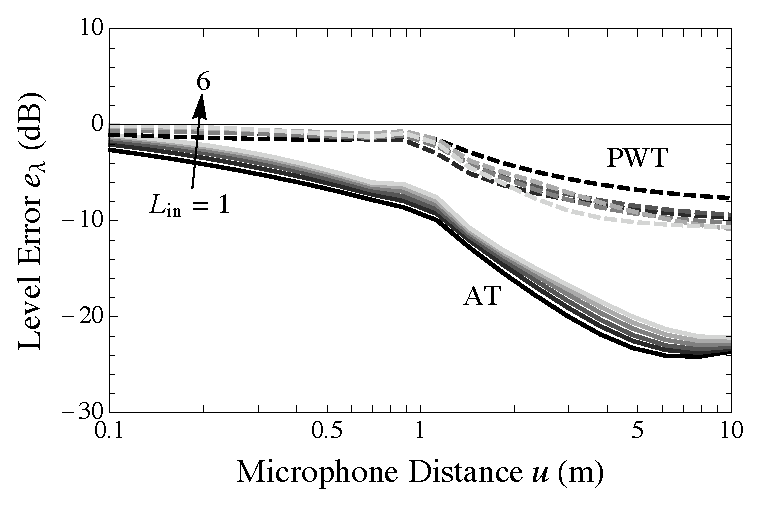
\includegraphics[width=\textwidth]{07_characterization_extrapolation/figures/audibleEnergy_order.eps}
        		\caption{Level errors $e_\lambda$}
        		\label{fig:07_Characterization_Extrapolation:Level_Errors:Order}
    	\end{subfigure}
	\hfill
    	\begin{subfigure}[b]{0.49\textwidth}
        		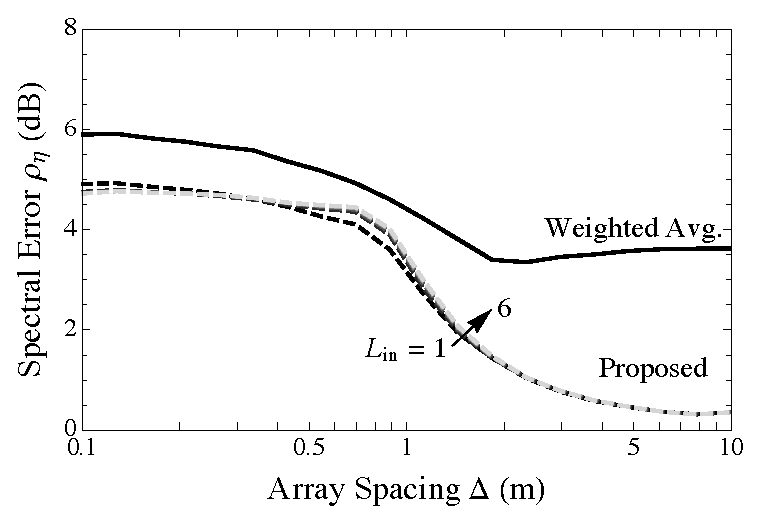
\includegraphics[width=\textwidth]{07_characterization_extrapolation/figures/scharer2009_order.eps}
        		\caption{Spectral errors $\rho_\eta$}
        		\label{fig:07_Characterization_Extrapolation:Spectral_Errors:Order}
    	\end{subfigure}
	
	\vspace{0.5cm}
	\begin{subfigure}[b]{0.49\textwidth}
        		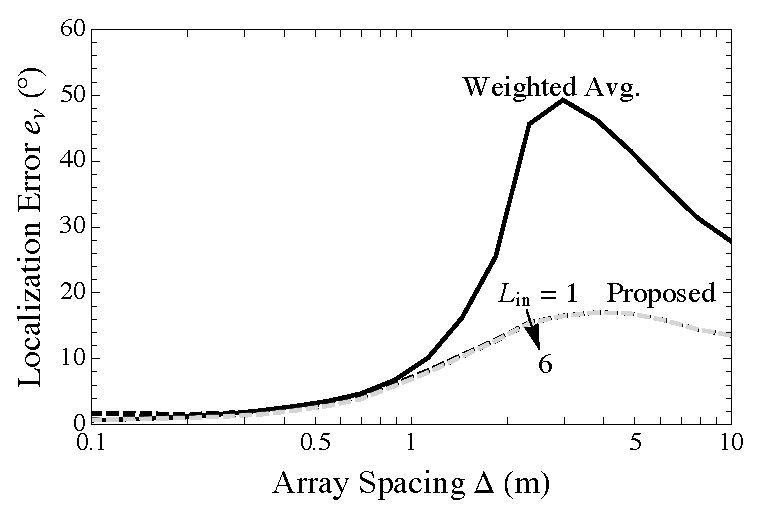
\includegraphics[width=\textwidth]{07_characterization_extrapolation/figures/tylka2017_order.eps}
        		\caption{Localization errors $e_\nu$}
		\label{fig:07_Characterization_Extrapolation:Localization_Errors:Order}
    	\end{subfigure}
	\hfill
    	\begin{subfigure}[b]{0.49\textwidth}
        		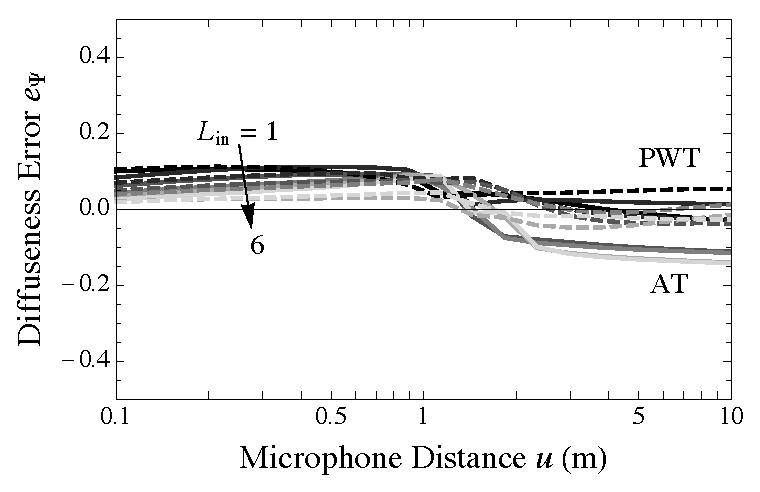
\includegraphics[width=\textwidth]{07_characterization_extrapolation/figures/merimaa2005_d_order.eps}
        		\caption{Diffuseness errors $e_\Psi$}
		\label{fig:07_Characterization_Extrapolation:Diffuseness_Errors:Order}
    	\end{subfigure}
	
    	\caption[Order dependence plots for each extrapolation method.]{
	Errors for various microphone distances $u$ with a fixed source distance $s_0 = 1$~m.
	Errors are plotted for the ambisonics translation method (solid curves, labeled ``AT'') and the plane-wave translation method (dashed curves, labeled ``PWT'').
	For each method, six input ambisonics orders are shown: $L_\textrm{in} = 1$ (black) to $L_\textrm{in} = 6$ (lightest gray).}
    	\label{fig:07_Characterization_Extrapolation:Order_Errors}
\end{figure*}

From \figref{fig:07_Characterization_Extrapolation:Spectral_Errors:Order}, we again see that increasing the ambisonics order $L_\text{in}$ yields an improvement in performance (i.e., a decrease in spectral errors) for the ambisonics translation method.
Here again we note two distinct regimes for this method on either side of $u = 1$~m with a transition region where the behavior changes.
Additionally, within each regime, the errors again increase monotonically with increasing $u$.
However, unlike with level errors, we now see a more rapid (but still monotonic) increase in error for \textit{exterior} sources ($u < 1$~m), while the more gradual performance degradation occurs for \textit{interior} sources ($u > 1$~m).
For the plane-wave translation method, we see that increasing $L_\text{in}$ yields an \textit{increase} in spectral error, and that this increase in error is more severe for interior sources than for exterior ones.
This suggests a penalty from violating the region of validity restriction that is particular to the plane-wave translation method: that a larger ambisonics input order incurs more spectral coloration.

As shown in \figref{fig:07_Characterization_Extrapolation:Localization_Errors:Order}, the localization errors for both methods tend to improve with increasing $L_\text{in}$, and the existence of two regimes on either side of $u = 1$~m is evident.
For exterior sources ($u < 1$~m), the errors improve with decreasing $u$, whereas for interior sources ($u > 1$~m), the opposite is true: the errors improve with \textit{increasing} $u$.
Evidently, a microphone distance of $u \approx s_0$ (i.e., $\gamma \approx 1$) yields the most extreme errors.
Overall, the ambisonics translation method tends to perform worse than the plane-wave translation method (except at very large $u$ and $L_\text{in} = 1$) and the errors for both methods are typically smaller for exterior sources than for interior ones.

It is worth noting that by construction, since $s_0$ is fixed, as $u$ increases beyond $1$~m, more of the navigable region (see \figref{fig:06_Simulation_Framework:Point_Geometry}) becomes valid for translation.
For instance, with $u = 10$~m and $s_0 = 1$~m, the listener can navigate approximately $9$~m away from the microphone and still remain inside its region of validity.
This explains in part the improvement with increasing $u$ seen for $u > 1$~m, since, on average, more of the navigable region is valid.
That is, when averaging errors over the entire navigable region, a smaller fraction of that region will actually be in violation of the region of validity restriction.

Finally, as shown in \figref{fig:07_Characterization_Extrapolation:Diffuseness_Errors:Order}, both methods achieve small diffuseness errors, and generally, increasing $L_\text{in}$ improves the performance for exterior sources.
Again we see a transition between regimes occurring at $u \approx 1$~m.